\chapter{Training, validation and test data}
In a classification problem, we divide the (usually manually) labeled dataset $D=\{(x_i,y_i)\}$ into three disjoint sets, including a training dataset $X$, a validation dataset $V$ and a test dataset $T$.
% to give an expectation of the real generalization of NN.

	\begin{enumerate}
		\item The labeled dataset $D=\{(x_i,y_i)\}_{i=1}^N$: $x_i$ are samples and $y_i$ are corresponding labels. For example, Figure \ref{xd:lbd} shows the labeled dataset of five class points, i.e. $x_i\in\mathbb{R}^2,y_i=1:5$.
		
			\begin{figure}[!ht] 
				\center{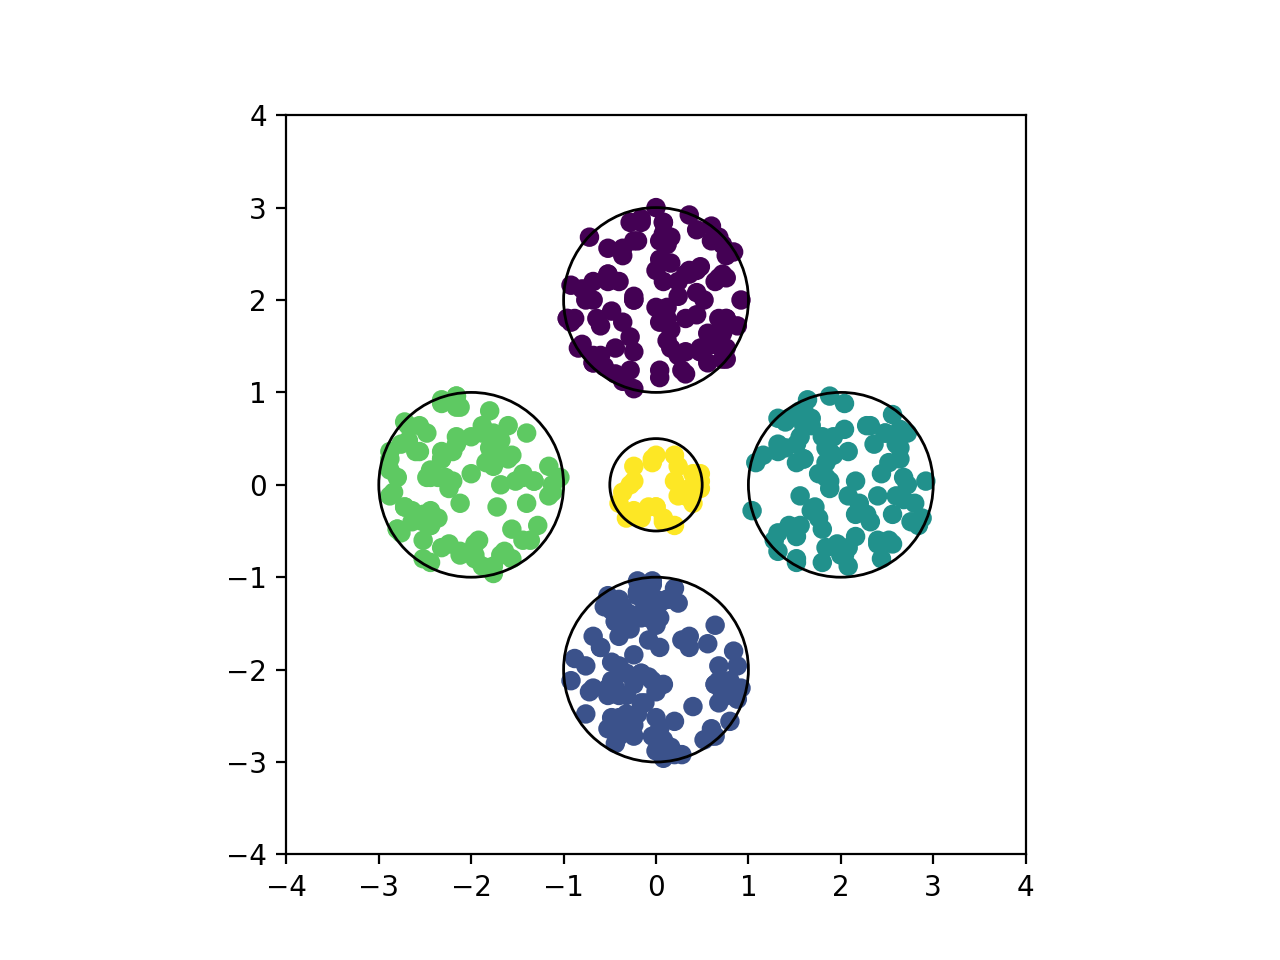
\includegraphics[width=10cm] {Homework1_5classes.png}}        
				\caption{labeled dataset} 
				\label{xd:lbd}
			\end{figure}
			 
		\begin{enumerate}
			\item Training Data $X$: we use it to train the neural network $f_\theta(x)$, aiming at minimizing the loss function $\mathcal{L}(X;\theta)$ by adjusting $\theta$.
			
			\item Validation Data $V$: 
			\begin{enumerate}
				\item Detecting whether the neural network is over-fitting, i.e. if $\mathcal{L}(X)$ decreases while $\mathcal{L}(V)$ increases.
				\item If it is the case, one may consider stopping training on $X$, because the prediction ability of $f_\theta$ on other samples (which are what we really want) may decrease.
				\item To make full use of the labeled data, one may continue to train $f_\theta$ with $V$, and make $X$ the validation data.
			\end{enumerate}
			\item Test Data $T$
			\begin{enumerate}
				\item Testing the real performance of $f_\theta$.
				\item We expect a similar accuracy on other unlabeled data as on the test data.
			\end{enumerate}
		\end{enumerate}
		
		\item Data augmentation: how to generate more data (to avoid over-fitting and make the training easier)
			\begin{enumerate}
				\item Shift: shift an image
				\item Rotation: rotate an image
				\item Crop: separate an image to small (intersected) images
				\item ...
			\end{enumerate}
	\end{enumerate}
	

